\documentclass[10pt,a4paper,twocolumn]{article}
\usepackage[margin=19mm,columnsep=7mm]{geometry}
\usepackage[T1]{fontenc}
\usepackage[utf8]{inputenc}
\usepackage{lmodern,amsmath,amssymb,booktabs,tabularx,enumitem,microtype,graphicx}
\usepackage[numbers,sort&compress]{natbib}
\usepackage[hidelinks]{hyperref}
\usepackage{xurl}
\setlength{\emergencystretch}{2em}
\renewcommand{\dbltopfraction}{0.85}
\renewcommand{\textfraction}{0.1}
\newcommand{\jeq}{\mathrel{=_{\mathrm{json}}}}
\newcommand{\jneq}{\mathrel{\neq_{\mathrm{json}}}}
\newcommand{\system}{\textsc{Auto-Decte}}
\newcommand{\context}{\mathrm{context}}
\newcommand{\bound}{\mathrm{bound}}
\hypersetup{pdftitle={Review-to-Execution Continuity for Corrected Agent State Changes},pdfauthor={Liang Hanghao; Xuan Wentao; Chen Qile; Peng Peng}}
\title{Review-to-Execution Continuity for Corrected Agent State Changes}
\author{Liang Hanghao \quad Xuan Wentao \quad Chen Qile \quad Peng Peng\\
\small College of Computer Science and Electronic Engineering, Hunan University\\
\small Changsha 410082, China; corresponding author: \texttt{hnu16pp@hnu.edu.cn}}
\date{}
\begin{document}
\maketitle
\begin{abstract}
State-changing agents may continue acting after a reviewer corrects and authorizes a proposal. An equivalent candidate can then replace the reviewed instance even when the final value is correct. We define correction-aware review-to-execution continuity through four roles: machine proposal, authorized correction, reviewed candidate and executed transition. An executable contract links them to predecessor freshness, atomic successors and field-level provenance. Formal checks, transactional realizations, controlled tests and archived correction chains establish complementary evidence. A frozen paired study over 128 tasks and two deployments, together with a separately frozen 117-pair deployment-A evaluation, measures continuity, recovery and execution costs. In standardized handoffs, all 16 original-B continuations receiving instance-mismatch feedback recover through reviewed-candidate reuse; all 15 supplementary-A continuations recover through reuse or fresh authorization. Their context counterparts admit substituted instances. For standardized handoff pairs, mean additional continuation costs are one tool call in original B and 1.60 in supplementary A. Agent-managed refreshed previews show no observed substitution, while completion uncertainty leaves the utility trade-off open. The contract constrains the authorized state change while allowing multiple legal recovery sequences, making continuity both enforceable and observable in subsequent agent execution.
\end{abstract}
\noindent\textbf{Keywords:} trustworthy agents; review-to-execution continuity; human authorization; transactional execution; provenance; agent recovery

\section{Introduction}
Agents that invoke tools increasingly change persistent operational state. They update records, publish revised values and commit results that later actions treat as authoritative. Trustworthy execution therefore requires an accountable connection between a state change and the review that authorized it. Human-in-the-loop frameworks already pause tool calls, permit argument edits and resume execution \citep{langchainHITL}. The open execution question is what must remain continuous while an agent acts after that review.

Correction makes this question concrete. A machine proposes $x_c$; a reviewer authorizes $x_a$. When a proposal of 100 is corrected to 101, the system should commit 101 and retain the original 100 as proposal evidence. Guided repair and interactive cleaning already distinguish system suggestions from human judgments \citep{yakout2011guided,he2016falcon}. In a state-changing agent workflow, the distinction extends across time: the system must retain both what was proposed and which reviewed instance is entitled to supply the later transition.

Suppose two persisted candidates, $c_1$ and $c_2$, propose 100 for the same field and retain the same evidence, producer and expected predecessor. They differ only in instance identity. A reviewer inspects $c_1$ and authorizes 101. The agent then obtains an equivalent preview, or receives a queued handoff carrying $c_2$, and executes it under the earlier grant. The value may still be 101. Every retained contextual check may agree. Under an instance-accountability requirement, however, the transition has crossed a review boundary: the candidate used for execution is not the one reviewed. Figure~\ref{fig:contract} separates value correctness from this review-to-execution relation.

Transactions, provenance and approval provide essential foundations. Transactions install atomic changes \citep{gray1981transaction}; concurrency control validates the predecessor \citep{kung1981occ}; provenance retains derivation and responsibility \citep{buneman2006curated,moreau2013provdm}; and authorization mechanisms bind approval to an executable request \citep{clark1987integrity,owaspTransactionAuthorization}. We make the reviewed instance an explicit execution constraint for corrected state updates, and isolate its operational consequences while holding the authorized value and retained context fixed. If enforcement rejects a continuation, its feedback becomes input to an agent that must choose a legal next step.

We ask: \emph{How should authorization preserve review-to-execution continuity when corrected agent proposals become persistent changes, and how does enforcement reshape subsequent execution and recovery?} Our answer combines an executable contract with a paired online intervention. The contract connects the four roles to freshness, complete successors and exact field sources. The intervention compares retained-context and instance-bound policies after the same reviewed history, following actual feedback through the next meaningful action, recovery path, task utility and integrity.

The paper makes four contributions:
\begin{enumerate}[leftmargin=*,itemsep=2pt]
\item \textbf{Correction-aware continuity.} We define the four-role review-to-execution relation and construct histories that separate equal values and retained context from the identity of the reviewed instance.
\item \textbf{An executable authorization contract.} We integrate instance binding with predecessor freshness, atomic complete successors and field-level provenance, supported by bounded formal checks and independent persistence auditing.
\item \textbf{Cross-layer mechanism evidence.} Controlled comparisons establish policy separation and agreement across two exact-binding realizations; request-binding tests and archived hosted-agent corrections connect the contract to its integration boundaries.
\item \textbf{Online execution and recovery evidence.} A frozen paired intervention and a separately frozen deployment-A evaluation measure how authorization feedback changes subsequent agent actions, while reporting utility, integrity and operational friction by collection cohort.
\end{enumerate}

Three findings organize the evidence. \textbf{Continuity}: a correct endpoint can retain the wrong reviewed origin. \textbf{Enforcement}: relational constraints and transactional effects expose and enforce that distinction. \textbf{Recovery}: original B and supplementary A recover through different legal paths with measurable friction. Agent-managed refreshed previews show no observed substitution.

\begin{figure*}[t]
\centering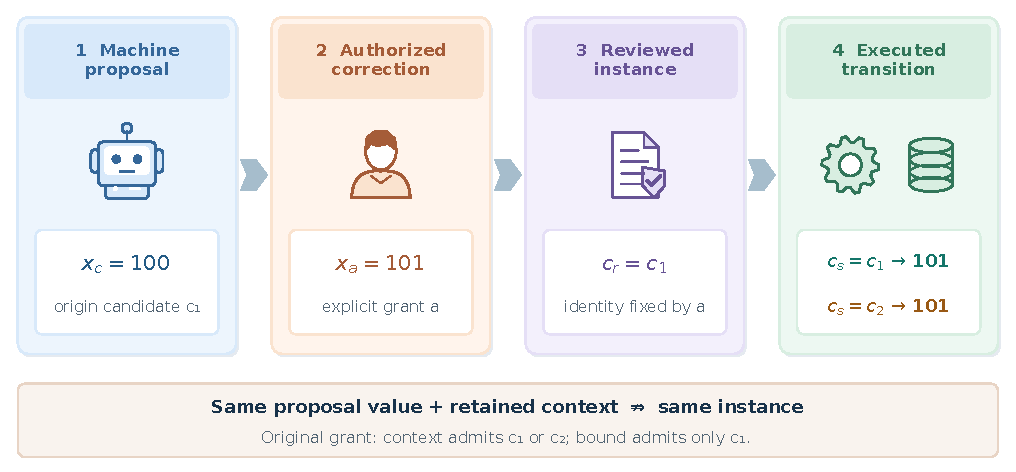
\includegraphics[width=\textwidth]{figures/revised-figure1-concept.pdf}
\caption{Correction-aware review-to-execution continuity. Review authorizes 101 from $c_1$ while retaining its proposal 100. Equivalent $c_2$ has the same value/context but a different identity. Context permits either instance under the original grant; bound permits only $c_1$. A new authorization can license $c_2$. This is a conceptual construction.}
\label{fig:contract}
\end{figure*}

\section{Related Work}
\subsection{Agent approval and tool execution}
Approval mechanisms already control state-changing operations. Clark--Wilson combines authenticated execution, well-formed transactions and reconstructible audit records \citep{clark1987integrity}. Collaborative databases can retain cell versions pending approval, including approval tied to a cell identifier and timestamp \citep{mershad2015approval}. Current agent middleware interrupts selected tool calls and permits approval, edits or rejection before resumption \citep{langchainHITL}. Server-controlled authorization data and a final execution gate are established security guidance \citep{owaspTransactionAuthorization}. Our correction case concerns the relation among four roles after such a decision: the original proposal, the corrected authorized value, the reviewed candidate and the candidate used for execution. A completed approval step provides a starting point for that relation; the continuation determines whether it is preserved.

\subsection{Transactions, provenance and \mbox{governed} state}
Transactions and optimistic concurrency control support atomic successors and validation against current state \citep{gray1981transaction,kung1981occ}. Database provenance identifies contributing data and derivations \citep{buneman2001whywhere,cheney2009provenance}. Curated-database provenance records edits and copies across versions, including the connection of unchanged data to preceding versions \citep{buneman2006curated}; reenactment reconstructs transaction provenance \citep{arab2018reenactment}. PROV-DM models entities, activities, agents and their responsibility relations \citep{moreau2013provdm}. These mechanisms supply the persistence vocabulary for the execution contract. The authorization target still has to specify whether equivalent contents or a particular reviewed instance may supply a corrected transition. We implement the same contract with relational objects and an event journal so that this question is separated from storage representation.

\subsection{Trustworthy execution and \mbox{recovery}}
AgentDojo separates task utility from security outcomes in interactive tool environments \citep{debenedetti2024agentdojo}. Table~\ref{tab:authorization-comparison} compares nearby authorization and recovery mechanisms. Prior work already binds proposal identity and supports recovery. Our intervention fixes the corrected value and retained context while varying whether execution must use the reviewed instance. It separates machine proposal, authorized replacement and reviewed/executed identities, then measures subsequent actions, recovery paths and costs.

\begin{table*}[t]
\centering
\small
\caption{Conceptual comparison of authorization boundaries and reported continuation evidence, not a cross-system benchmark.}
\label{tab:authorization-comparison}
\begin{tabularx}{\textwidth}{@{}>{\raggedright\arraybackslash}p{0.20\textwidth}>{\raggedright\arraybackslash}p{0.32\textwidth}>{\raggedright\arraybackslash}X@{}}
\toprule
Work & Approval or binding focus & Reported continuation evidence \\
\midrule
LangChain HITL \citep{langchainHITL} &
Selected tool calls and arguments; approve, edit or reject. &
Documented checkpointed resumption, execution of edited calls and rejection feedback. \\
\addlinespace
Cordon \citep{chen2026cordon} &
Task transaction, result lineage, staged effects and scoped approval. &
Containment benchmarks and deterministic rollback/resume checks; released external effects require audit or compensation. \\
\addlinespace
Continuity Kernel \citep{he2026continuity} &
Proposal identity, exact predecessor, pre-state authority and evidence bound to activation. &
Bounded invariant checks and forward restoration under current authority. \\
\addlinespace
Commit-time authorization \citep{santosgrueiro2026committime} &
Witness freshness, causal priority, effect binding and eligibility at durability. &
Controlled invalidation separates endpoint success from authorized completion; guarded abort and witness-revalidation recovery. \\
\addlinespace
This work &
Machine proposal, corrected value, reviewed instance and executed transition. &
Paired instance-policy contrast after the same review; observed reuse/reauthorization, utility, integrity and continuation costs. \\
\bottomrule
\end{tabularx}
\end{table*}

\section{Review-to-Execution \mbox{Continuity}}
\subsection{Four roles in a corrected state change}
Let $\Sigma_v$ be an authoritative record state with a nonempty field domain $F_r$, total values $V_v:F_r\to X$ and total durable sources $S_v:F_r\to T$. A persisted candidate is
\begin{equation}
c=\langle id,r,f,e,v_{\rm exp},x_c,p\rangle,
\end{equation}
where $id$ names the immutable instance, $r,f$ identify the target, $e$ identifies persisted evidence and its locator, $v_{\rm exp}$ is the expected predecessor, and $p$ identifies the producer. Retained context $K(c)$ includes the declared non-identity review information. Instance identity is not reconstructed from the proposal value or $K(c)$.

An authorization $a=\langle c_r,x_a,q\rangle$ records the reviewed instance $c_r$, explicit authorized value $x_a$ and authorized principal $q$, together with its validity information. A commit request submits $c_s$ and a value $x$. The roles obey
\begin{align}
\operatorname{proposal}(c_r)&=x_c,\nonumber\\
\operatorname{authorized}(a)&=x_a,\nonumber\\
\operatorname{committed}(\Sigma_{v+1},f)&\jeq x_a.
\end{align}
For illustration, a record has quantity 90 and batch \texttt{B-008} sourced from $t_b$. Candidate $c_1$ proposes 100; review authorizes 101. The successor contains quantity 101 through $t_1$ and the unchanged batch with exact source $t_b$. Correction permits $x_c\jneq x_a$; $c_1$ retains 100. In the online facade, successful commit consumes the grant: identical arguments with the same idempotency key return the prior receipt without a new transition; a new key under the consumed grant is rejected as semantic replay. Online Resource 1, Section S3 develops this construction, which is not an additional experiment.

Contract value comparisons use canonical JSON equality, written $\jeq$: sorted-key, whitespace-minimal serialization must agree. Thus integer \texttt{101} and floating serialization \texttt{101.0} are distinct values; Booleans also remain distinguishable when their serialization differs. Change detection, admission value checks, tracing and the independent oracle share this equality.

\subsection{Content agreement and reviewed-instance continuity}
For an already issued authorization, define
\begin{align}
K_{eq}&\iff K(c_s)=K(c_r),\nonumber\\
I_{eq}&\iff id(c_s)=id(c_r).
\end{align}
Let $G$ collect the remaining disclosed checks: authorization validity, predecessor freshness, committed-value equality, evidence integrity, successor shape, source relations, transaction constraints and grant consumption. It excludes an implicit instance comparison. The two execution policies are
\begin{align}
P_\context&: \operatorname{Admit}=G\land K_{eq},\label{eq:context}\\
P_\bound&: \operatorname{Admit}=G\land K_{eq}\land I_{eq}.\label{eq:bound}
\end{align}
Both retain the reviewed identifier. Only the decision to require its equality at execution differs. Context-equivalent $c_2$ can therefore pass Eq.~\ref{eq:context} under $c_1$'s authorization while failing Eq.~\ref{eq:bound}. This is a policy separator under a declared instance-accountability requirement. Context-based authorization remains a coherent choice for an application whose responsibility contract treats those instances as interchangeable.

\subsection{Failure-distinguishing information}
To identify which distinctions the contract must retain, the declared failure model separates five information classes: candidate identity/context ($D_C$), proposal/authorized-value attribution ($D_V$), predecessor freshness ($D_F$), complete atomic successor ($D_B$), and total field sources ($D_S$). For a history $h$, $\pi_I(h)$ retains the specified logical observations in $I$, and $O(h)$ assigns the full-history authority outcome, including successor and trace status. Candidate handles are opaque: a reduced observation cannot recover an omitted class by decoding an identifier.

\paragraph{Proposition 1: class-wise irredundancy.}
For every $d\in\mathcal D=\{D_C,D_V,D_F,D_B,D_S\}$, the declared model contains paired histories satisfying
\begin{equation}
\pi_{\mathcal D\setminus\{d\}}(h_s)=\pi_{\mathcal D\setminus\{d\}}(h_u),
\quad O(h_s)\ne O(h_u).
\end{equation}
Thus a decision based on the reduced observations cannot distinguish both required outcomes.

\paragraph{Construction.}
Hold the other observations fixed while changing, respectively, candidate/context binding, the authority assigned to a corrected value, the entry-time predecessor comparison, the single-versus-fragmented commit sequence, or one required source anchor. Each pair changes the corresponding derived authority outcome. A fixed-registry pair further selects either the reviewed candidate or a context-equivalent alternative while retaining the same two candidates and non-identity information. It isolates instance continuity within $D_C$. Observation functions and valid histories are specified independently; the checker derives projections and outcomes from complete relations. This establishes class-wise irredundancy within the declared failure model. Full constructions and projection assumptions are in the supplement.

\subsection{Atomic successors and exact source preservation}
For an admitted nonempty batch $B$ with unique changed fields, the required effects are
\begin{equation}
\Delta(V_v,V_{v+1})=\{i.f:i\in B\}=\{t.f:t\in T_{v+1}\}.
\end{equation}
Each admitted item has one transition to its explicitly authorized value; all items share the target record, observed predecessor and one successor. Initial coverage establishes complete value/source domains. Later admissions preserve every unchanged field's value and exact source:
\begin{equation}
f\notin\Delta\Rightarrow V_{v+1}(f)\jeq V_v(f),\quad S_{v+1}(f)=S_v(f).
\end{equation}
Decision, authorization binding, transitions, complete version, sources and audit effects commit together, or the authoritative state stutters. This multi-field guarantee is single-record; cross-record or distributed atomicity is not validated. Candidate and review preparation already persisted before the attempted admission remain historical evidence. Online Resource 1, Section S2 states the full P0--P6 contract, no-op handling and mixed-submission semantics.

\section{Formal and Transactional \mbox{Realization}}
\subsection{Making the relation executable}
The relational model encodes candidates, evidence, principals, authorizations, ordered versions, complete states and source transitions. Machine events may extend candidates and evidence while framing authoritative state. Full admission adds binding, freshness, complete shape and item--transition correspondence to the base state change. Removing a conjunct while retaining another valid item exposes which required distinction that conjunct enforces. Alloy and Kodkod make these finite relational checks executable \citep{jackson2002alloy,torlak2007kodkod}. The independent concrete-to-relational mapping follows the abstraction/concretization testing principle exemplified by TestEra \citep{marinov2001testera}.

The archived checks cover legal admissions, conjunct-removal witnesses, source attacks and nonempty trace-preservation premises. All 72 command outcomes agree with their manifests across two scope profiles. The assertion checks have no counterexamples within their encoded finite scopes. An independent abstraction reads persisted pre/post relations, maps them into fixed instances, and checks Full admission or rejected-state stutter: nine intended projections are satisfiable and twenty selected mapping mutants are unsatisfiable. The supplement records exact scopes, commands, assumptions and concrete/formal domain differences.

\subsection{Transactional persistence and review binding}
\system{} separates candidate-writing capability from authoritative admission. An immutable certificate includes the persisted candidate instance and its canonical target, proposal, producer, expected predecessor and evidence identity. A review decision binds that certificate to the explicit authorized value. Field transitions retain the chain through both accepted and corrected proposals.

The relational adapter reloads the current field domain, complete predecessor, evidence and authorization within the transaction. It derives changed fields using canonical equality, validates exact bindings and unused identities, checks the principal policy, and compares-and-swaps the expected version. It then writes one transition per admitted field and copies exact unchanged sources into one complete successor. Constraints reinforce unique transitions and coherent references. Rejected admissions and transactions aborted before commit make no authoritative state change; a committed transition is not undone by a subsequently unavailable response.

A separately implemented event journal stores the same authority-relevant relations. Its retained-context configuration omits instance equality at the execution gate; its exact configuration adds the reviewed-candidate link. Comparing the exact journal with the relational implementation tests the same contract across storage representations. Comparing the two journal configurations isolates the binding choice within one representation.

Faithful transfer of review requires a binding before the final request arrives. A server-held review record can fix the candidate, expected version, reviewer and corrected value, then validate the request against that record. The resulting guarantee concerns request-to-record consistency. Browser presentation is a separately observable layer: a page can display a different candidate while the server and request still name the recorded one. Controlled request and display probes identify that boundary.

\subsection{Independent audit of authoritative effects}
The source verifier follows every field through its exact transition, authorization, candidate certificate, producer, evidence and predecessor. Changed fields need their unique new transition; unchanged fields retain the preceding source. A separate database oracle reads persisted relations rather than trusting the production planner or trace builder. Rejection checks compare full logical database digests, and corruption probes require changed state plus a diagnosis. These checks connect the written contract to the actual durable successor.

The prospective experiment uses another independent oracle for the paired policies. It checks raw responses against executed tool actions, hash-linked events, persisted state snapshots and reviewed-history provenance. Integrity is determined from authoritative transitions and audit coverage, rather than from a gate's own claim that an operation was admissible. This permits a context-admitted transition to satisfy its policy while violating the separately declared instance-continuity oracle.

\section{Controlled and Historical Evidence}
\subsection{Controlled mechanism and system validation}
Context-equivalent substitutions separate reviewed-instance continuity from content approval. The archived E1 comparison executes 165 cases per mechanism. The context journal accepts all fifteen same-value/same-context substitutions; the exact journal and relational reference reject them. The two exact mechanisms agree on all corresponding decisions and provenance-query answer sets. Each accepts 45 legal cases and rejects 120 with authoritative-state stutter. This establishes the executable separator that the online experiment subsequently turns into agent-visible feedback.

\begin{table}[t]
\centering\small
\caption{Controlled mechanism evidence. Counts retain their original interpretation units; all cases are constructed or scripted.}
\label{tab:controlled}
\begin{tabularx}{\columnwidth}{@{}lX@{}}
\toprule
Evidence & Observed result \\
\midrule
Persistence binding & Exact journal/reference agree in 165 cases; context accepts 15 instance substitutions \\
Request binding & Server-held gate rejects 9 request substitutions accepted by original path \\
Display boundary & Both paths accept 3 display-only substitutions \\
Formal/concrete checks & 72 bounded commands match; 9 intended projections SAT; 20 mapping mutants UNSAT \\
\bottomrule
\end{tabularx}
\end{table}

Server-held review binding separates request substitution from faithful presentation. E2 has thirty browser cases per path: nine legitimate controls, nine request substitutions, nine stale/replay/interrupted controls and three display-only substitutions. The gate rejects every request substitution while preserving the legitimate controls. Both paths reject the stale, replay and interrupted cases without fact writes. Both admit the display-only controls because their actual request still matches the server record. Table~\ref{tab:controlled} groups this evidence under one realization question.

The persistence contract also makes implementation cost measurable. Complete confirmation and source reconstruction are timed separately, with exact output agreement checked across the 36 paired trace-workload cells. Online Resource 1, Section S4 separates single-record admission timings from trace workloads varying field count, history depth and background record population. Agent-level friction is measured after the online policy intervention, where the additional work is an observed part of continuation.

\subsection{Observable correction in hosted workflows}
The correction contract is recoverable from archived hosted-agent persistence. A new audit of 1,260 historical databases identifies 84 retained machine-origin correction chains, checking 252 evidence associations, 168 record versions and 168 reconstructed provenance traces. Each chain preserves a machine proposal, explicit host-authorized correction, exact candidate binding and persisted transition. These chains provide integration evidence for the role distinction defined in Section 3.

The audit unit is a persisted correction chain rather than whole-task success. The corresponding archived endpoints include 80 strict-safe task successes, one safe utility failure, two model/API failures and one timeout. All 84 persisted chains satisfy the audited relation. Their single-field cases provide zero unchanged-field checks, so copy-forward is supported by the controlled multi-field evidence. Full original task and annotation denominators remain in the supplement, separate from the prospective policy experiment.

\section{Prospective Online Agent Experiment}
Controlled mechanism separation establishes that the policies differ, but it does not tell us what happens once that difference becomes feedback to an adaptive agent. The prospective experiment compares Eqs.~\ref{eq:context} and \ref{eq:bound} in live continuations. It is designed around the sequence
\begin{equation}
\begin{aligned}
\text{feedback}&\to\text{next agent action}\\
&\to\text{recovery path}\to(U,I).
\end{aligned}
\end{equation}
The local precollection freeze fixes the tasks, pair order, deployments, prompts, tools, resource rules, scorer and failure handling. The separately archived pilot supports engineering readiness and is excluded from formal effect analysis.

The online evaluation comprises the original frozen collection and a separately frozen supplementary paired evaluation of deployment A. To extend post-review continuation coverage, the latter selects the 117 tasks whose original prefixes ended with quota-exhaustion errors before receiving a model response. It retains the task inputs, prompts, tools, policy order, requested deployment configuration and scoring rules, and evaluates recovery paths and execution costs in a later collection period. All planned arms and attempt histories are retained; the original 512-arm analysis remains unchanged, and each collection has its own reporting denominator.

\subsection{Shared review history and unique policy difference}
A shared prospective prefix isolates the post-review continuation effect by giving both policies the same reviewed history (Figure~\ref{fig:loop}). An actual agent proposes and obtains host review; the complete visible conversation and persisted state are then copied into isolated policy arms. The same task, checkpoint, tools, deterministic reviewer, persistence, prompt and resource-policy family apply to both arms. This isolates the effect of requiring $I_{eq}$ on subsequent continuation. Both arms retain the reviewed identifier, so the comparison changes its use at execution rather than its availability for auditing.

A deterministic host reviewer fixes the correction decision across arms, separating authorization consequences from variation in review judgments. Configuration A requests \texttt{gpt-5.6-terra} through account-backed Codex CLI \texttt{0.160.1} with low reasoning; the CLI exposes no returned model identifier. Configuration B requests \texttt{deepseek-v4-flash} through DeepSeek's Anthropic-compatible Messages API at temperature zero and receives the same identifier. Neither route exposes an immutable model revision. Both use the same serialized JSON action interface: the model selects an action, which the host executes before returning its actual result to the next decision. Complete settings and collection timestamps are retained in Online Resource 1 and the artifact.

Each task/configuration forms one adjacent context/bound pair. A frozen assignment manifest balances which policy runs first within scenario and configuration. The original collection uses two provider lanes, each executing one pair at a time; the supplementary evaluation uses one A lane, respecting the same pair order. All planned arms remain in the analysis ledger, with runtime outcomes and audit coverage recorded separately. The supplement specifies the collection and interruption rules.

\begin{figure*}[t]
\centering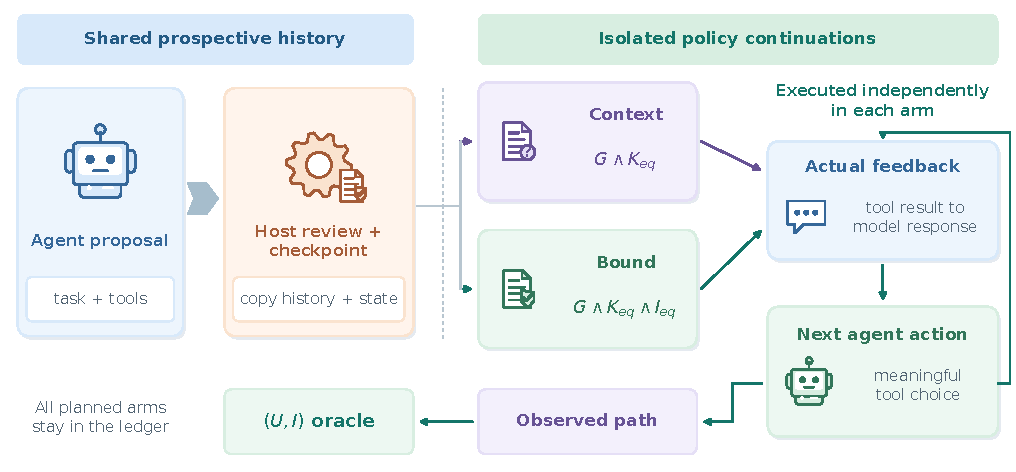
\includegraphics[width=\textwidth]{figures/revised-figure3-online-loop.pdf}
\caption{Paired online intervention after a shared prospective review. The visible conversation and persisted checkpoint are copied into isolated policy arms. The only execution-rule difference is $I_{eq}$. Actual tool feedback enters the next sampled agent decision, whose actions and terminal state are independently audited. The standardized G handoff supplies an index request; N instead leaves refreshed-preview management to the agent.}
\label{fig:loop}
\end{figure*}

\subsection{Task families and controlled exposure}
The original design contains 128 task instances, two configurations and two policies: 256 paired units and 512 planned policy trajectories, with one repetition. Controlled correction tasks expose specific authorization boundaries while keeping legal recovery paths interpretable. Their frozen distribution is
\[
L32+N32+G16+E16+V16+R16=128.
\]
The constructed workflows correct quantities or monetary amounts in purchase, inventory and reconciliation records. In frozen task \texttt{FORMAL-G-001}, the instruction is to review the source snapshot and correct record \texttt{P2F-FORMAL-G-001}'s quantity: the predecessor contains 3379, ERP evidence supports proposal 3368, and the host reviewer authorizes 3367. The goal preserves the purchase memo, business context, history and their sources while updating quantity to 3367.

\begin{description}[leftmargin=0pt,itemsep=2pt]
\item[L: legal correction.] Execute the reviewed instance with the corrected authorized value; check ordinary completion and nonvacuous unchanged-source preservation.
\item[N: refreshed preview.] After authorization, the agent obtains a required refreshed preview and decides how to preserve continuity. It can reuse the reviewed instance, authorize a new candidate or otherwise manage the workflow; the harness does not force an invalid commit.
\item[G: queued handoff.] The harness creates a same-value/same-context new instance and performs one standardized index action under the prior grant. It repeats \texttt{propose}, preserving target/field, proposal value, predecessor, evidence identity/bytes/hash/locator, template/schema, producer/selection metadata and parent links. A fresh candidate identifier and recomputed certificate lie outside $K$, yielding $K_{eq}$ with unequal instance identity. The actual result becomes feedback for autonomous continuation. The index action is marked \texttt{harness\_handoff}; it is a standardized recovery probe.
\item[E: changed evidence.] Publish changed evidence bytes and locator while preserving the proposal value. Both policies enforce the shared evidence/context checks; recovery can obtain a candidate reviewed against current evidence.
\item[V: stale predecessor.] Advance authoritative state externally. A fresh-state read, proposal and authorization provide a legal recovery path while preserving the externally updated source.
\item[R: unavailable receipt.] After a successful commit, the first receipt path is unavailable while authoritative state remains readable. Distinguish state confirmation, exact idempotent retry and semantic replay of a consumed grant.
\end{description}
The task generator varies business template, correction direction/magnitude, value relations, evidence layouts/locators, sources, version/history depths, retained metadata, candidate envelopes, snapshot organization, ordering and task wording. All 128 parameter vectors and rendered inputs are frozen. These variations diversify instances while preserving the six mechanisms.

\subsection{Utility, integrity and recovery}
Task utility $U=1$ requires the authoritative goal, required workflow actions and an accurate final report. Integrity is independently scored as $I\in\{1,0,\mathrm{unknown}\}$. Covered authoritative transitions must satisfy authorization, freshness, evidence/context integrity, authorized-value equality, provenance, copy-forward and the declared instance-continuity requirement. A proved violation yields $I=0$; incomplete necessary evidence yields unknown unless a violation is already proved. Runtime failure or rejected execution does not alone determine integrity.

Joint outcomes retain $(U,I)=(1,1),(1,0),(0,1),(0,0)$ and integrity unknown. A policy-admissible context substitution can therefore complete the task while failing the instance oracle. Completion and integrity are never collapsed into a total score.

A rejection is recoverable when its feedback is delivered and a legal path exists at the recorded rejection-time state. Delivery requires an actual received next model response with the recorded feedback input. Recoverability is determined from that state and available capabilities, not inferred backward from eventual success. The event-order classifier records the next meaningful tool action and observed reuse, verification, reproposal, reauthorization, state/evidence refresh, repeated invalid attempts, abandonment, confirmation and terminal failure. Raw component actions remain available alongside the primary path label. Every $U=0$, $I=0$ or unknown arm enters the complete failure-archaeology ledger.

\subsection{Paired effects and operational components}
Two primary endpoints are frozen: $\Delta U=U_\bound-U_\context$ and the bound-minus-context difference in run-level instance-continuity failure incidence. Transition-level executed substitution is a separate diagnostic. Unknown continuity contributes explicit identification bounds rather than a zero replacement.

For original aggregate effects, each task contributes its average configuration-specific paired difference. A scenario-stratified bootstrap resamples 128 task clusters, retaining both configurations and both policies; the frozen plan uses 10,000 iterations and seed 20261007. Separate configuration-specific exact McNemar tests are secondary. The structure supplies paired effects and controlled-task uncertainty, rather than 512 independent samples. Supplementary A effects are an exploratory application of this bootstrap procedure to its 117 selected task pairs; Section S12 gives their cohort-specific estimator and uncertainty. They do not replace the original two-deployment estimand.

Recovery distributions conditional on delivered rejection are descriptive because exposure is post-treatment. G-bound provides the standardized probe cohort; N remains a separate account of agent-managed continuity. Operational components report additional tool calls, model turns, authorization attempts, reproposals, verifications, elapsed time and observed provider usage. Unsuccessful runs retain the specified budget-capped time-to-success alongside their actual termination time. Shared-prefix provider usage is charged once per pair. No arbitrary composite friction score is introduced.

\section{Results}
Instance binding converts standardized candidate substitutions into accountable recovery in both original deployment B and supplementary deployment A. Their observed repair paths differ, while their median paired execution costs are similar. Table~\ref{tab:joint} reports checkpoint coverage and joint outcomes for each cohort.

\subsection{Continuity at execution}
A correct endpoint does not establish the reviewed origin of a state change. In original B, context admits sixteen instance substitutions; fourteen of these arms complete their tasks. In supplementary A, context admits fifteen substitutions and all fifteen arms complete. The corresponding bound handoffs reject the substituted instances and end with $(U,I)=(1,1)$. The same separation also appears in the single exposed original A pair. No proved continuity violation occurs outside G or under bound.

\begin{table*}[t]
\centering\small
\caption{Checkpoint coverage and joint task/integrity outcomes by collection. Planned and CP count pairs; each policy has one arm per pair. CP=reviewed checkpoint reached. The two unknown N arms belong to original B.}
\label{tab:joint}
\setlength{\tabcolsep}{3.8pt}
\begin{tabular}{@{}lrrlrrrrrr@{}}
\toprule
Collection & Planned & CP & Policy & $U=1,I=1$ & $U=1,I=0$ & $U=0,I=1$ & $U=0,I=0$ & $I$ unknown & $U=1$ \\
\midrule
Original A & 128 & 11 & Context & 8 & 1 & 119 & 0 & 0 & 9 \\
Original A & 128 & 11 & Bound & 9 & 0 & 119 & 0 & 0 & 9 \\
Original B & 128 & 128 & Context & 103 & 14 & 8 & 2 & 1 & 117 \\
Original B & 128 & 128 & Bound & 119 & 0 & 8 & 0 & 1 & 119 \\
Supplementary A & 117 & 117 & Context & 99 & 15 & 3 & 0 & 0 & 114 \\
Supplementary A & 117 & 117 & Bound & 116 & 0 & 1 & 0 & 0 & 116 \\
\bottomrule
\end{tabular}
\end{table*}

With 17 proved context violations and one unknown arm per policy, the original bound-minus-context continuity-failure difference lies in $[-7.03,-6.25]$ percentage points. Section S11 reports bootstrap uncertainty for these identification endpoints. Supplementary A has complete integrity coverage; its fifteen context violations and zero bound violations correspond to $-12.82$ points within its selected 117-pair cohort. These substitutions are admissible under the context policy and incompatible with the independent instance oracle. Their remaining evaluated evidence, value, freshness and provenance checks hold, locating the difference in the disclosed continuity obligation.

\subsection{Feedback, next actions and recovery paths}
Delivered instance-mismatch feedback exposes two legal routes to accountable execution. All sixteen original B continuations first commit the original reviewed candidate under its existing grant. All fifteen supplementary A continuations also recover: eight first reuse the reviewed candidate and seven first request authorization for the handoff candidate, then commit it. Feedback is proved delivered to an actual subsequent model response, and a legal path exists at each rejection state. The contract constrains the authorized state change without prescribing a single recovery sequence.

Original A's single delivered mismatch also recovers through fresh authorization (Online Resource 1, Section S11). Figure~\ref{fig:followup} compares original B and supplementary A. Recovery distributions are conditional on delivered feedback; they do not estimate naturally occurring mismatch prevalence.

\begin{figure*}[t]
\centering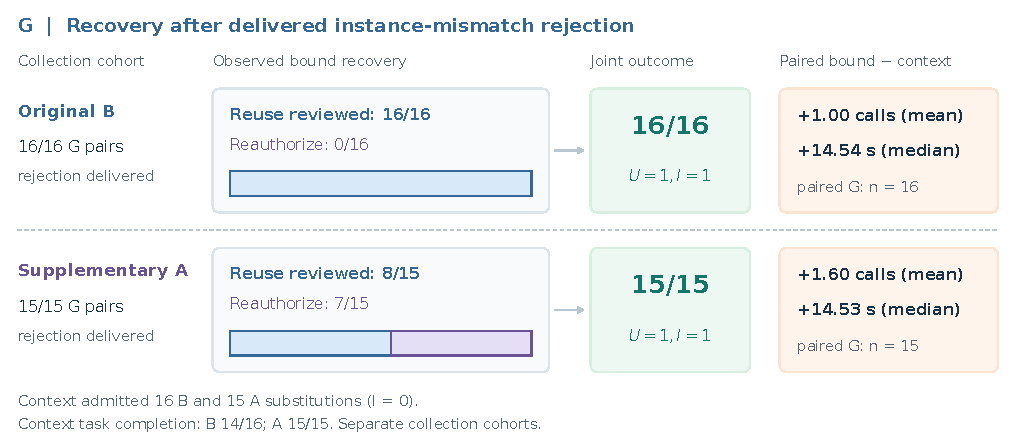
\includegraphics[width=\textwidth]{figures/followup-behavior-comparison.pdf}
\caption{Accountable recovery and paired execution costs at the standardized G boundary. Original B contributes 16 delivered G-bound mismatch episodes and supplementary A contributes 15; all end with $U=1,I=1$. B uses reviewed-candidate reuse throughout; supplementary A uses reuse in eight cases and reauthorization in seven. Calls are means and seconds are medians of bound-minus-context differences across the corresponding G task pairs, measured over the complete suffix.}
\label{fig:followup}
\end{figure*}

Agent-managed refreshed previews preserve reviewed-instance continuity in every covered N transition under either policy. Original B supplies thirty such transitions per policy, original A three and supplementary A twenty-nine. No delivered instance-mismatch feedback occurs in N. Original B completes 28/32 N arms per policy, with three covered unsuccessful arms and one unknown; supplementary A completes 29/29 per policy. Thus the observed behavioral consequence of the unique policy conjunct is concentrated in standardized G handoffs rather than voluntary preview management.

The shared boundaries elicit different repairs. In original B, changed evidence yields fifteen recoveries from sixteen delivered episodes per policy, stale predecessors twelve from thirteen, and unavailable receipts nine state-confirmation endpoints per policy. In supplementary A, changed evidence yields twelve recoveries from fourteen context and twelve bound episodes; stale predecessors yield seven from seven per policy. Receipt feedback yields fourteen context and thirteen bound state-confirmation recoveries; the remaining bound episode still ends in accurate task completion without a recorded recovery endpoint. Sections S11--S12 retain first actions, component labels and unsuccessful continuations, keeping episode recovery distinct from terminal utility.

\subsection{Task completion under paired authorization}
The original completion effect is small relative to its task-cluster uncertainty. Context completes 126/256 arms (49.22\%) and bound 128/256 (50.00\%). The frozen task-averaged bound-minus-context effect is $+0.78$ percentage points, with 95\% interval $[-1.95,3.52]$. Original B has 117/128 versus 119/128 completions, an effect of $+1.56$ points with interval $[-3.91,7.03]$; the secondary exact McNemar test gives $p=0.774$. Original A has nine completions under each policy.

The supplementary paired evaluation of deployment A completes 114/117 context arms and 116/117 bound arms. Its exploratory paired effect is $+1.71$ percentage points, with scenario-stratified 95\% bootstrap interval $[0.00,4.27]$ and secondary exact McNemar $p=0.50$. Section S12 reports the complete supplementary table and Section S13 a separately labeled post hoc sensitivity analysis. Neither estimate establishes a general completion improvement.

\subsection{Operational friction and retained failures}
Accountable recovery adds observable execution work at the G boundary. Original B's sixteen pairs use a mean and median of one extra suffix agent tool call, with no extra authorization requests; median additional suffix time is 14.54 seconds (mean 8.84). Supplementary A's fifteen pairs have a median of one extra call (mean 1.60) and median additional suffix time of 14.53 seconds (mean 17.97). Its seven reauthorization paths add a review request as well as a commit. Figure~\ref{fig:followup} uses paired whole-suffix costs, which also retain other differences in the continuation rather than equating the repair sequence with the entire run.

Across original B's 127 pairs with two suffix records, mean extra calls are 0.071 and median extra elapsed time is 0.69 seconds. Its budget-capped time-to-success endpoint retains all 128 pairs and has mean paired difference $-9.74$ seconds. In G that mean is $-76.53$ seconds despite positive median elapsed friction: two unsuccessful context reports receive the 720-second cap while all bound reports complete. Capped time and actual latency therefore answer different questions. Sections S11--S12 retain calls, turns, review requests, actual time, capped time and native usage separately, charging each shared prefix once.

The original ledger has 273 arms with $U=0$, $I=0$ or unknown integrity; supplementary A has nineteen, comprising fifteen successful but instance-violating context arms and four unsuccessful arms with intact covered integrity. Three of the latter have runtime terminations and one has an agent-final abandonment. The underlying events and states, including the deployment-identity check failure, remain available in Sections S11--S12. These observations distinguish availability, task completion and transition integrity without folding them into a composite score.

\section{Discussion and Limitations}
\subsection{What continuity adds to corrected execution}
Successful but instance-violating trajectories show that endpoint correctness does not establish reviewed origin. Instance authorization supplies that missing execution constraint alongside atomicity, predecessor validation and provenance. Agreement between relational and journal realizations, and the hosted-chain audit, show that this relation is enforceable and reconstructible across the evaluated persistence boundaries.

Retaining the reviewed candidate has an operational benefit beyond traceability: it makes reuse under the existing grant available as a legal next step. Fresh authorization provides a different route for the new candidate. Systems should preserve these usable objects and grants alongside the record that review occurred.

\subsection{Authorization as part of the execution environment}
The G comparison separates a mechanical policy difference from an agent's subsequent choice. The same standardized request is accepted or rejected; delivered feedback then leads to reviewed-candidate reuse or fresh authorization. The observed mixture in supplementary A and uniform reuse in original B demonstrate available legal paths, rather than a fixed workflow imposed by the gate.

The contrast with N clarifies the mechanism's place in an agent system. A refreshed preview creates the possibility of identity substitution but does not force the agent to exploit it. Covered N transitions preserve the reviewed instance even when the looser policy would accept a context-equivalent alternative. The contract therefore performs two functions: it documents accountability when the agent already maintains continuity and supplies actionable feedback when a queued handoff breaks it. An execution-layer benefit can be material even when voluntary mismatch is absent in the agent-managed cohort.

The broader recovery results also separate obligations from repair sequences. Changed evidence calls for a current evidence-based proposal and review; a stale predecessor calls for a current-state proposal; an unavailable receipt can be resolved by confirming state rather than applying another mutation. These paths use the same tool vocabulary but solve different contract boundaries. A useful execution environment should expose which relation failed and retain the state needed for a legal next step. Rejection frequency alone omits whether the agent received that information, acted on it and reached an accountable outcome.

\subsection{Accountability and execution cost}
Instance accountability adds execution work at the standardized handoff boundary. Original B's reuse requires one post-rejection commit; supplementary A also uses fresh authorization. Whole-suffix costs include these actions and other continuation differences, so the similar median latencies describe the recorded collection conditions. Systems can control which recovery capabilities and reusable authorizations remain available.

The original completion interval allows modest improvement or loss; the exploratory supplementary interval also includes zero. Capped time-to-success, actual latency and provider availability measure different outcomes. Calls, turns, review requests and $U/I$ should therefore remain separately reported: a covered run can preserve state while accomplishing nothing.

\subsection{Scope and further evaluation}
The 128 tasks provide controlled exposure to six execution boundaries, with one repetition per task/configuration/policy combination. The deterministic reviewer fixes correction and authorization decisions, isolating execution binding from variation in human judgment. These controlled effects do not estimate production mismatch prevalence; broader workflows with interactive reviewers would test transferability and review burden.

The supplementary A cohort was selected by its original availability state and collected later. The observed A/B recovery mixtures combine deployment and collection conditions, so they do not isolate differences in model capability. Requested aliases and settings support route reconstruction, but A's unexposed returned model revision limits exact response reproduction. Retained inputs, responses, checkpoints and independent scores support retrospective verification within that scope.

\section{Conclusion}
Correction-aware review-to-execution continuity separates what an agent proposed, what a reviewer authorized, which candidate was reviewed and which supplied a persistent transition. Formal relations, transactional realization and independent auditing make that distinction executable across persistence representations. Controlled and historical evidence establish the mechanism and its observable integration roles.

The online evaluations connect the contract to live continuation. Original B and supplementary A both complete every delivered standardized instance-mismatch recovery with intact continuity, using reviewed-candidate reuse or fresh authorization; their context counterparts admit the substituted instances. Agent-managed preview tasks produce no observed substitutions. Recovery adds measurable execution work, while completion uncertainty leaves the utility trade-off open. Enforced inside an agent loop, review-to-execution continuity becomes actionable feedback that redirects execution and exposes the cost of accountability.

\section*{Statements and Declarations}
\subsection*{Data and software availability}
The study uses constructed tasks and public lifecycle inputs. The controlled experiment archive is fixed at commit \href{https://github.com/lhh666-6/auto-dete/tree/2645e5e18c900ea91c9c980e44195dc71e410432/DKE-supplement}{\nolinkurl{2645e5e18c900ea91c9c980e44195dc71e410432}}. The reference implementation, formal models and earlier historical evidence are retained at commit \href{https://github.com/lhh666-6/auto-dete/tree/c6d512843c905cab6d8521dd8c914f7fb26d85ae/latest}{\nolinkurl{c6d512843c905cab6d8521dd8c914f7fb26d85ae}}. The prospective inputs and runner are fixed at master hash \nolinkurl{7773563b40c8db30d6def121915f50fbad032537edde32afd4ba39ec3eea744b}. The handoff archive at commit \href{https://github.com/lhh666-6/auto-dete/tree/475e66f549613aaaaa62c2ec81ffdee483636c54/cloud-handoff}{\nolinkurl{475e66f549613aaaaa62c2ec81ffdee483636c54}} retains the complete original formal ledger, raw responses, state snapshots, scorer, tables, figure sources and file hashes; Online Resource 1 maps the layers and reproduction steps. The accompanying supplementary evaluation package preserves its separate freeze, complete attempt history, independent scores and source hashes; Online Resource 1, Section S12 identifies the offline analysis entry point. Reanalysis requires no new model calls. New hosted runs require provider access. A \href{https://github.com/lhh666-6/auto-dete/blob/kais-reproducibility-2026-10-07/REPRODUCIBILITY.md}{fixed-version reproduction guide} provides the ordered offline workflow.

\subsection*{Ethics approval and consent to participate}
The prospective experiment uses constructed tasks and a deterministic host reviewer, with no new human participants. In the historical annotation study, one author (X.W.) and one non-author volunteer independently coded benign completion outcomes; L.H. adjudicated their disagreement and separately reviewed eleven human--rule disagreements. X.W. also completed the textual-acknowledgment annotation. Only pseudonymous annotator identifiers were collected. Both coders were informed of the task and data use, and the non-author coder participated voluntarily. The authors assessed the annotation of generated outputs as not requiring ethics approval. No animal subjects were involved.

\subsection*{CRediT authorship contribution statement}
Liang Hanghao: Conceptualization, Methodology, Software, Formal analysis, Investigation, Data curation, Validation, Visualization, Project administration, Writing--original draft, and Writing--review \& editing. Xuan Wentao: Methodology, Formal analysis, Investigation, Data curation, Validation, Visualization, and Writing--review \& editing. Chen Qile: Investigation and Validation. Peng Peng: Supervision and Writing--review \& editing.

\subsection*{Funding and competing interests}
This research received no external funding. The authors declare no competing interests.

\subsection*{AI-assisted preparation}
DeepSeek and OpenAI tools, including Codex, were used to assist with code development, analysis checks, literature organization, figure preparation, and manuscript drafting and revision. The authors retain full responsibility for the research design, interpretation of the results, and the accuracy and integrity of the final manuscript.

\subsection*{Supplementary information}
Online Resource 1 contains formal constructions and checks, full controlled workloads, historical records, prospective task and deployment definitions, scoring and interruption rules, complete outcome and recovery tables, and the artifact map.

\begin{thebibliography}{99}
\bibitem{langchainHITL} LangChain. Human-in-the-loop. Official documentation. \url{https://docs.langchain.com/oss/python/langchain/human-in-the-loop}. Accessed 7 October 2026.
\bibitem{yakout2011guided} Yakout M, Elmagarmid AK, Neville J, Ouzzani M, Ilyas IF (2011) Guided data repair. Proc VLDB Endow 4(5):279--289. \url{https://doi.org/10.14778/1952376.1952378}.
\bibitem{he2016falcon} He J, Veltri E, Santoro D, Li G, Mecca G, Papotti P, Tang N (2016) Interactive and Deterministic Data Cleaning. Proc SIGMOD, pp 893--907. \url{https://doi.org/10.1145/2882903.2915242}.
\bibitem{gray1981transaction} Gray J (1981) The Transaction Concept: Virtues and Limitations. Proc Seventh International Conference on Very Large Data Bases, pp 144--154.
\bibitem{kung1981occ} Kung HT, Robinson JT (1981) On optimistic methods for concurrency control. ACM Trans Database Syst 6(2):213--226. \url{https://doi.org/10.1145/319566.319567}.
\bibitem{buneman2006curated} Buneman P, Chapman A, Cheney J (2006) Provenance management in curated databases. Proc SIGMOD, pp 539--550. \url{https://doi.org/10.1145/1142473.1142534}.
\bibitem{moreau2013provdm} Moreau L, Missier P (eds) (2013) PROV-DM: The PROV Data Model. W3C Recommendation. \url{https://www.w3.org/TR/2013/REC-prov-dm-20130430/}.
\bibitem{clark1987integrity} Clark DD, Wilson DR (1987) A Comparison of Commercial and Military Computer Security Policies. IEEE Symposium on Security and Privacy, pp 184--194. \url{https://doi.org/10.1109/SP.1987.10001}.
\bibitem{owaspTransactionAuthorization} OWASP Foundation. Transaction Authorization Cheat Sheet. \url{https://cheatsheetseries.owasp.org/cheatsheets/Transaction_Authorization_Cheat_Sheet.html}. Accessed 7 October 2026.
\bibitem{mershad2015approval} Mershad K, Malluhi QM, Ouzzani M, Tang M, Aref WG (2015) Approving Updates in Collaborative Databases. IEEE International Conference on Cloud Engineering, pp 42--47. \url{https://doi.org/10.1109/IC2E.2015.31}.
\bibitem{buneman2001whywhere} Buneman P, Khanna S, Tan WC (2001) Why and Where: A Characterization of Data Provenance. ICDT, LNCS 1973, pp 316--330. \url{https://doi.org/10.1007/3-540-44503-X_20}.
\bibitem{cheney2009provenance} Cheney J, Chiticariu L, Tan WC (2009) Provenance in Databases: Why, How, and Where. Found Trends Databases 1(4):379--474. \url{https://doi.org/10.1561/1900000006}.
\bibitem{arab2018reenactment} Arab BS, Gawlick D, Krishnaswamy V, Radhakrishnan V, Glavic B (2018) Using Reenactment to Retroactively Capture Provenance for Transactions. IEEE Trans Knowl Data Eng 30(3):599--612. \url{https://doi.org/10.1109/TKDE.2017.2769056}.
\bibitem{debenedetti2024agentdojo} Debenedetti E, Zhang J, Balunovic M, Beurer-Kellner L, Fischer M, Tram\`er F (2024) AgentDojo: A Dynamic Environment to Evaluate Prompt Injection Attacks and Defenses for LLM Agents. Advances in Neural Information Processing Systems 37:82895--82920. \url{https://doi.org/10.52202/079017-2636}.
\bibitem{chen2026cordon} Chen Z, Liu H, Xu D, Dong D, Li J, Pu B, Zhai J (2026) Cordon: Semantic Transactions for Tool-Using LLM Agents. arXiv preprint arXiv:2606.17573v1. \url{https://doi.org/10.48550/arXiv.2606.17573}.
\bibitem{he2026continuity} He J, Yu D (2026) Beyond Memory: A Transactional Continuity Kernel for Long-Lived AI Agents. arXiv preprint arXiv:2608.11632v1. \url{https://doi.org/10.48550/arXiv.2608.11632}.
\bibitem{santosgrueiro2026committime} Santos-Grueiro I (2026) Temporary Authority, Permanent Effects: Commit-Time Authorization for LLM Agents. arXiv preprint arXiv:2607.10487v1. \url{https://doi.org/10.48550/arXiv.2607.10487}.
\bibitem{jackson2002alloy} Jackson D (2002) Alloy: a lightweight object modelling notation. ACM Trans Softw Eng Methodol 11(2):256--290. \url{https://doi.org/10.1145/505145.505149}.
\bibitem{torlak2007kodkod} Torlak E, Jackson D (2007) Kodkod: A Relational Model Finder. TACAS, LNCS 4424, pp 632--647. \url{https://doi.org/10.1007/978-3-540-71209-1_49}.
\bibitem{marinov2001testera} Marinov D, Khurshid S (2001) TestEra: A Novel Framework for Automated Testing of Java Programs. IEEE International Conference on Automated Software Engineering, pp 22--31. \url{https://doi.org/10.1109/ASE.2001.989787}.
\end{thebibliography}
\end{document}
